% $Id$
%
\usebackgroundtemplate{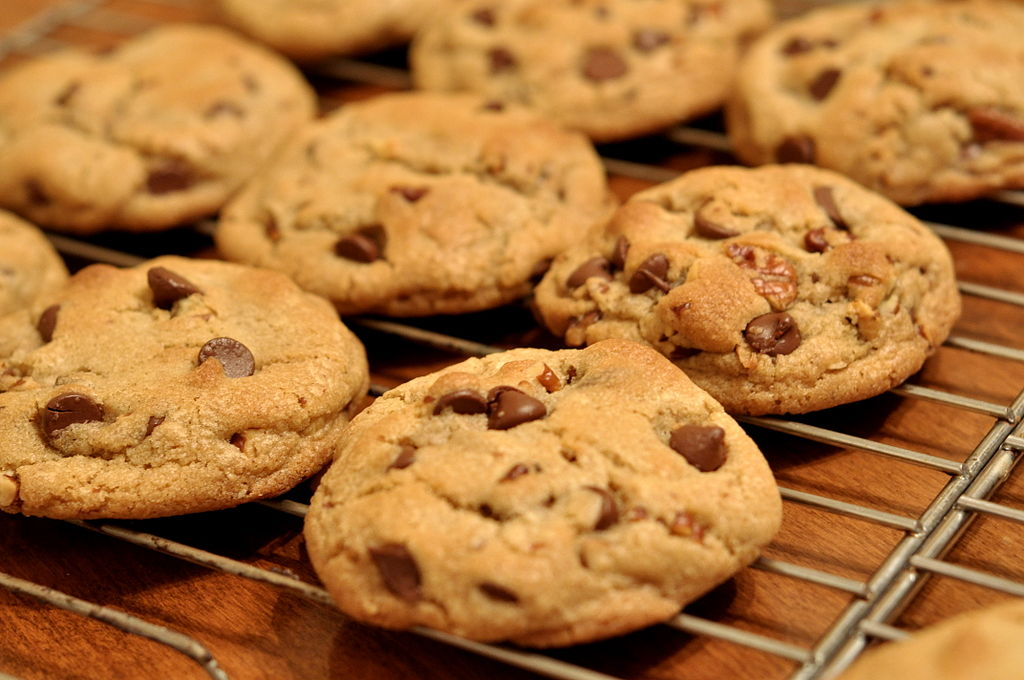
\includegraphics[width=13cm]{figs/cookies.jpg}}
% Original figure: Wikipedia
% http://upload.wikimedia.org/wikipedia/commons/thumb/b/b9/Chocolate_Chip_Cookies_-_kimberlykv.jpg/1024px-Chocolate_Chip_Cookies_-_kimberlykv.jpg
{\bf
  \textcolor[rgb]{1,1,1}{
    \section{Cookies HTTP}
  }
}

%%---------------------------------------------------------------
\usebackgroundtemplate{}

\begin{frame}
\frametitle{Cookies}

\begin{itemize}
\item Forma de mantener estado en un protocolo sin estado (HTTP)
\item Forma de almacenar datos en el lado del cliente
\item Dos versiones principales:
  \begin{itemize}
  \item Versi�n 0 (Netscape)
  \item Version 1 (RFC 2109 / RFC 2965)
  \end{itemize}
\end{itemize}
\end{frame}


%%---------------------------------------------------------------
\begin{frame}[fragile]
\frametitle{Cabeceras HTTP para cookies (version 0)}

\begin{itemize}
\item Set-Cookie: De servidor a navegador \\

\begin{verbatim}
  Set-Cookie: statusmessages="deleted"; Path=/; 
    Expires=Wed, 31-Dec-97 23:59:59 GMT
\end{verbatim}

\begin{itemize}
\item Nombre de la cookie: statusmessages
\item Valor: "deleted"
\item Path: / (todo el sitio del que se recibi�)
\item Expira: 31-Dec-97 23:59:59 GMT
\end{itemize}

\item Cookie: De navegador a servidor \\

\begin{verbatim}
  Cookie: statusmessages="deleted"
\end{verbatim}

\begin{itemize}
\item Nombre de la cookie: statusmessages
\item Valor: "deleted"
\end{itemize}

\end{itemize}

RFC 2965 (version 1) tiene: ``Cookie'', ``Cookie2'' y ``Set-Cookie2''
\end{frame}

%%---------------------------------------------------------------
\begin{frame}
\frametitle{Estructura de Set-Cookie}

\begin{itemize}
\item Nombre y valor (obligatorios)
  \begin{itemize}
  \item Uso normal: ``nombre=valor''
  \item Tambi�n valor nulo: ``nombre=''
\end{itemize}
\item Fecha de expiraci�n
  \begin{itemize}
  \item ``Expires=fecha''
  \item Si no tiene, cookie no persistente (s�lo en memoria)
  \end{itemize}
\item Path: camino para el que es v�lida
  \begin{itemize}
  \item ``Path=/camino''
  \item Prefijo de caminos v�lidos
  \end{itemize}
\item Domain: dominio para el que es v�lida
  \begin{itemize}
  \item El servidor ha de estar en el dominio indicado
  \item Si no se indica, servidor que sirve la cookie
  \end{itemize}
\item Seguridad: se necesita SSL para enviar la cookie
  \begin{itemize}
  \item Campo ``Secure'' 
  \end{itemize}
\item Campos separados por ``;''
\end{itemize}
\end{frame}

%%---------------------------------------------------------------
\begin{frame}[fragile]
\frametitle{Estructura de Cookie}

\begin{itemize}
\item Lista de pares nombre - valor
\item Cada par corresponde a un ``Set-Cookie''
\item Se env�an las cookies v�lidas para el dominio y el path de la petici�n HTTP
\item Si no se especific� dominio en ``Set-Cookie'', el del servidor
\item Si no se especific� camino en ``Set-Cookie'', todo
\end{itemize}

\begin{verbatim}
Cookie: user=jgb; last=5; edited=False
\end{verbatim}

\end{frame}

%%---------------------------------------------------------------
\begin{frame}
\frametitle{L�mites para las cookies}

\begin{itemize}
\item Originalmente: 20 cookies del mismo dominio
\item La mayor�a de los navegadores: 30 o 50 cookies del mismo dominio
\item Cada cookie: como mucho 4 Kbytes
\end{itemize}


\end{frame}

%%---------------------------------------------------------------
\begin{frame}[fragile]
\frametitle{Gesti�n de sesi�n en HTTP}

\begin{itemize}
\item Mediante cookies: normalmente, identificador de sesi�n en la cookie

\begin{verbatim}
Set-Cookie: session=ab34cd-34fd3a-ef2365
\end{verbatim}

\item Reescritura de urls: se a�ade identificador a la url

\begin{verbatim}
http://sitio.com/path;session=ab34cd-34fd3a-ef2365
\end{verbatim}

\item Campos escondidos en formularios HTML

\begin{verbatim}
<form method="post" action="http://sitio.com/path">
  <input type="hidden" name="session" value="ab34cd-34fd3a-ef2365">
  ...
  <input type="submit">
</form>
\end{verbatim}

\end{itemize}

\end{frame}


%%---------------------------------------------------------------
\begin{frame}
\frametitle{Referencias}

\begin{itemize}
\item Persistent Client State HTTP Cookies \\
  (especificaci�n original de Netscape) \\
  \url{http://curl.haxx.se/rfc/cookie_spec.html}
\item RFC 2109: HTTP State Management Mechanism \\
  \url{http://tools.ietf.org/html/rfc2109}

\item RFC 2965: HTTP State Management Mechanism \\
  \url{http://tools.ietf.org/html/rfc2965}
\end{itemize}
\end{frame}
